%% LyX 2.0.2 created this file.  For more info, see http://www.lyx.org/.
%% Do not edit unless you really know what you are doing.
\documentclass[english]{beamer}
\usepackage{mathptmx}
\usepackage[T1]{fontenc}
\usepackage[latin9]{inputenc}
\usepackage{color}
\usepackage{calc}
\usepackage{amsmath}
\usepackage{amssymb}
\usepackage{graphicx}

\makeatletter

%%%%%%%%%%%%%%%%%%%%%%%%%%%%%% LyX specific LaTeX commands.
%% Because html converters don't know tabularnewline
\providecommand{\tabularnewline}{\\}
%% A simple dot to overcome graphicx limitations
\newcommand{\lyxdot}{.}


%%%%%%%%%%%%%%%%%%%%%%%%%%%%%% Textclass specific LaTeX commands.
 % this default might be overridden by plain title style
 \newcommand\makebeamertitle{\frame{\maketitle}}%
 \AtBeginDocument{
   \let\origtableofcontents=\tableofcontents
   \def\tableofcontents{\@ifnextchar[{\origtableofcontents}{\gobbletableofcontents}}
   \def\gobbletableofcontents#1{\origtableofcontents}
 }
 \long\def\lyxframe#1{\@lyxframe#1\@lyxframestop}%
 \def\@lyxframe{\@ifnextchar<{\@@lyxframe}{\@@lyxframe<*>}}%
 \def\@@lyxframe<#1>{\@ifnextchar[{\@@@lyxframe<#1>}{\@@@lyxframe<#1>[]}}
 \def\@@@lyxframe<#1>[{\@ifnextchar<{\@@@@@lyxframe<#1>[}{\@@@@lyxframe<#1>[<*>][}}
 \def\@@@@@lyxframe<#1>[#2]{\@ifnextchar[{\@@@@lyxframe<#1>[#2]}{\@@@@lyxframe<#1>[#2][]}}
 \long\def\@@@@lyxframe<#1>[#2][#3]#4\@lyxframestop#5\lyxframeend{%
   \frame<#1>[#2][#3]{\frametitle{#4}#5}}
 \def\lyxframeend{} % In case there is a superfluous frame end

%%%%%%%%%%%%%%%%%%%%%%%%%%%%%% User specified LaTeX commands.
\usetheme{WAC}
% or ...

\setbeamercovered{transparent}
% or whatever (possibly just delete it)

\makeatother

\usepackage{babel}
\begin{document}
\setbeamercolor{normal text}{bg=yellow!10}

%\setbeameroption{show notes}


\title[LAMS Applications]{Calibrating Pressure, Dynamic Pressure, and Temperature Using a Laser
Air Motion Sensing System}


\author[Al Cooper]{Al Cooper\\
}


\institute[NCAR EOL]{\vskip-4cm\includegraphics[scale=0.07]{/home/cooperw/Documents/Work/Images/EOLlogo}\\
RAF Algorithm Review}


\date[]{December 2 2011}

\makebeamertitle

\note[item]{example note}



%\pgfdeclareimage[height=0.5cm]{institution-logo}{institution-logo-filename}

%\logo{\pgfuseimage{institution-logo}}
\pgfdeclareimage[height=0.5cm]{institution-logo}{/home/cooperw/Documents/Work/NSFReviewTalk/EOLlogo}

\logo{\pgfuseimage{institution-logo}}







%\beamerdefaultoverlayspecification{<+->}

\setbeamercolor{alerted text}{fg=red}


\lyxframeend{}\section{Roadmap}


\lyxframeend{}\lyxframe{ROADMAP}
\begin{columns}%{}


\column{5.5 cm}


\vskip-0.3cm
\begin{block}
{Steps:}
\begin{enumerate}
\item <+-|alert@+|visible@+->$p_{t}=p+q$ is accurate
\item <+-|alert@+|visible@+->Errors in $p$ and $q$ arise from error at
static sources
\item <+-|alert@+,8,9|visible@+->Find $\Delta q$ required to match LAMS;
hence $\Delta p$
\item <+-|alert@+|visible@+->Refinements for accuracy
\item <+-|alert@+,8,9|visible@+->$\Delta p$ is a function of measured
quantities like $p_{m}$, $q_{m}$, $\alpha_{m}$
\item <+-|alert@+,10|visible@+->Test using flight maneuvers, also calibrating
$T$
\item <+-|alert@+,11|visible@+->Use LAMS with the above results to measure
$T$ directly.
\end{enumerate}
\end{block}

\column{5.5 cm}
\begin{onlyenv}%{}
<1>
\begin{summaryblock}
{$p_{t}$}
\begin{itemize}
\item $p_{t}$=total pressure, $p$=static, $q=$dynamic
\item pitot tube insensitive to flow angle (<0.1\%)
\item orientation removes normal offset
\item redundant measurements $\Rightarrow$consistency
\item still, AN ASSUMPTION
\end{itemize}
\end{summaryblock}
\end{onlyenv}%{}


\begin{onlyenv}%{}
<2>
\begin{summaryblock}
{Consequences}
\begin{itemize}
\item $p$ and $q$ are the measured quantities
\item plumbing: $q$ is difference, $q=p_{t}-p$
\item therefore $\Delta p=-\Delta q$
\item can predict $q$ from LAMS, hence $\Delta q$
\item can use $\Delta p$ to correct $p$
\end{itemize}
\end{summaryblock}
\end{onlyenv}%{}


\begin{onlyenv}%{}
<4>
\begin{summaryblock}
{Adjustments}
\begin{itemize}
\item correct because $p$ enters the prediction of $\Delta p$
\item calculate humidity influences on $R_{a}$, $C_{p}$, $C_{v}$, $\gamma=c_{p}/c_{v}$
\item correct for offset angle of LAMS
\item recalculate $T$ using corrected pressures
\end{itemize}
\end{summaryblock}
\end{onlyenv}%{}


\begin{onlyenv}%{}
<5>
\begin{summaryblock}
{Fit Correction to $p$ and $q$ given by LAMS:}
\begin{itemize}
\item use second-by-second prediction of $\Delta q$ from LAMS
\item try fits like $(\Delta p/p)=a_{0}+a_{1}q+a_{2}(ADIFR/QCR)$
\item find $\Delta p(measurements)$
\end{itemize}
\end{summaryblock}
\end{onlyenv}%{}


\begin{onlyenv}%{}
<6>
\begin{summaryblock}
{Maneuvers for testing results}
\begin{itemize}
\item reverse-heading maneuvers
\item climbs and descents to calibrate temperature via integration of the
hydrostatic equation
\end{itemize}
\end{summaryblock}
\end{onlyenv}%{}


\begin{onlyenv}%{}
<7>
\begin{summaryblock}
{LAMS-based measurement of temperature}
\begin{itemize}
\item LAMS provides TAS=$v$
\item $p$ and $q$ determine Mach number $M=v/v_{s}$
\item $v_{s}=\sqrt{\gamma R_{a}T}$ so measured $M$ and $v$ $\Rightarrow$$T$
without reference to a temperature sensor
\end{itemize}
\end{summaryblock}
\end{onlyenv}%{}


\begin{onlyenv}%{}
<3>
\begin{summaryblock}
{What $q$ is required to match LAMS?}
\begin{itemize}
\item TAS: depends on $q$, $p$, $T$
\item relatively insensitive to $T$ (iterate...)
\item find $\Delta q$ s.th. $q_{m}+\Delta q$, $p_{m}-\Delta q$, T gives
$v_{\mathrm{LAMS}}$
\end{itemize}
\end{summaryblock}
\end{onlyenv}%{}


\begin{onlyenv}%{}
<8->
\begin{summaryblock}
{Results:}
\begin{enumerate}
\item <+-|alert@+|visible@+->Calibration of dynamic pressure, hence true
airspeed, hence longitudinal component of wind 
\item <+-|alert@+|visible@+->Calibration of pressure
\item <+-|alert@+|visible@+->Calibration of temperature via accurate measurements
of pressure + GPS
\item <+-|alert@+|visible@+->Provide new independent temperature measurement
that $should$ work in cloud
\end{enumerate}
\end{summaryblock}
\end{onlyenv}%{}
\end{columns}%{}

\lyxframeend{}\section{Finding ``PCORRS''}


\lyxframeend{}\subsection{The Total Pressure ($p+q$) }


\lyxframeend{}\lyxframe{THE MEASUREMENT OF TOTAL PRESSURE}
\begin{columns}%{}


\column{5.2 cm}


\vskip-0.3 cm
\begin{block}
{Basic Measurements}

\framebox{\begin{minipage}[t]{0.95\columnwidth}%
\begin{description}
\item [{static~pressure}] PSFD, PSFRD \end{description}
\begin{itemize}
\item absolute sensors
\item $\pm0.1$ mb (Parascientific Model 1000)\end{itemize}
%
\end{minipage}}


\framebox{\begin{minipage}[t]{0.95\columnwidth}%
\begin{description}
\item [{dynamic~pressure}] QCF, QCRF\end{description}
\begin{itemize}
\item differential sensors, total vs static
\item $\pm0.05$ mb\end{itemize}
%
\end{minipage}}


\framebox{\begin{minipage}[t]{0.95\columnwidth}%
\begin{description}
\item [{hypothesis:}] ~~
\end{description}
~~~~~~~~~~$p_{t}=p+q$ is accurate%
\end{minipage}}

\end{block}




\column{6.5 cm}
\begin{onlyenv}%{}
<2>
\begin{exampleblock}
{pitot tube performance}
\begin{itemize}
\item typical sensitivity <1\% at angles up to 10$^{\circ}$, 0.2\% up to
5$^{\circ}$.
\item mean orientation chosen along expected flow direction, not centerline
\end{itemize}
\end{exampleblock}
\end{onlyenv}%{}


\begin{onlyenv}%{}
<3>

\vskip-4cm


\centerline{PSFRD+QCFR=$a_1$(PSFD+QCF)+$a_2$}
\centerline{$a_1$=1.0000, $a_2$=0.10 mb}


\begin{center}
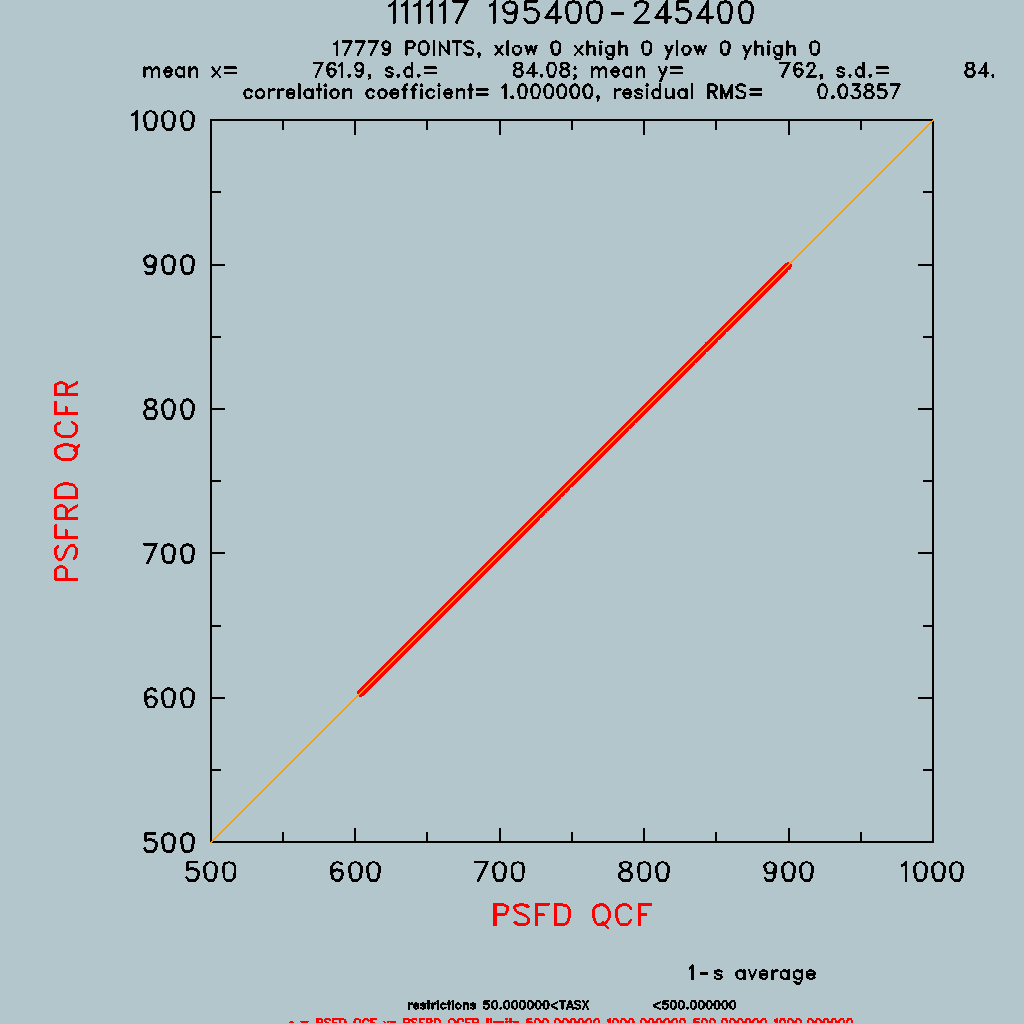
\includegraphics[width=0.9\columnwidth]{/home/cooperw/Xanadu/IDEAS/TotalPressure}
\par\end{center}


\vskip-5.5cm \hskip1,5cm\fcolorbox{black}{yellow!40}{%
\begin{minipage}[c][1\totalheight][t]{0.33\columnwidth}%
RMS scatter: 0.04 mb%
\end{minipage}}

\end{onlyenv}%{}
\end{columns}%{}

\lyxframeend{}\subsection{Finding $\Delta p$ using LAMS}


\lyxframeend{}\lyxframe{THE EQUATIONS}

Energy conservation in compressible flow:~~~~$\frac{v^{2}}{2}+c_{p}T=\mathrm{constant}$

For adiabatic compression to stagnation ($v=0)$, 

\[
M^{2}=\frac{v^{2}}{\gamma R_{a}T}=\left\{ \left(\frac{2c_{v}}{R_{d}}\right)\left[\left(\frac{p+q}{p}\right)^{R_{a}/c_{p}}-1\right]\right\} 
\]


\[
q=p{\color{red}\left\{ \left(\frac{v^{2}}{2c_{p}T}+1\right)^{c_{p}/R_{a}}-1\right\} }=p{\color{red}\chi}
\]


where the last equality defines $\chi(v,T).$ Write in terms of measured
quantities $p_{m}=p-\Delta p$ and $q_{m}=q-\Delta q$ and unknown
$\Delta p=-\Delta q$:

\begin{center}
\vskip-0.8cm\fcolorbox{black}{yellow!40}{%
\begin{minipage}[t]{0.27\columnwidth}%
\begin{center}
\[
\Delta p=\frac{q_{m}-p_{m}\chi}{1+\chi}
\]

\par\end{center}%
\end{minipage}}
\par\end{center}


\lyxframeend{}\lyxframe{HOW TO ADDRESS NEED FOR TEMPERATURE}
\begin{columns}%{}


\column{5.5 cm}
\begin{block}
{Need Temperature:}

Have $v$ from LAMS


\[
\chi({\color{red}v},{\color{blue}T})=\left\{ \left(\frac{{\color{red}v^{2}}}{2c_{p}{\color{blue}{\color{blue}T}}}+1\right)^{c_{p}/R_{a}}-1\right\} 
\]

\begin{itemize}
\item Not very sensitive: Fractional error in $T$ is small
\item Use available-processed $T$ as the first approximation
\item Then, iterate both in calculation and in calibration
\end{itemize}
\end{block}




\column{6 cm}
\begin{alertblock}
{Determining "PCORR" Function}

\begin{center}
\fcolorbox{black}{yellow!40}{%
\begin{minipage}[t]{0.5\columnwidth}%
\begin{center}
\[
\Delta p=\frac{q_{m}-p_{m}\chi}{1+\chi}
\]

\par\end{center}%
\end{minipage}}
\par\end{center}
\begin{itemize}
\item Airspeed from LAMS gives second-by-second estimates of $\Delta p$
\item Can fit those values to get $\Delta p$ as function of other measure-
ments
\end{itemize}
\end{alertblock}
\end{columns}%{}

\lyxframeend{}\lyxframe{REFINEMENTS FOR ACCURACY}
\begin{block}
{Moist Air Corrections}
\begin{itemize}
\item humidity matters at this level of precision
\item Use $R_{a}$, $c_{p}$, $\gamma$ adjusted for humidity
\end{itemize}
\end{block}
\begin{exampleblock}
{Pointing Angle Corrections}
\begin{itemize}
\item $v_{l}=v\,\cos(\theta)$ where $v_{l}$ is the speed measured by LAMS
\item $\cos\theta\simeq\cos(\theta_{1}+\alpha)\cos(\theta_{2}-\beta)$ 

\begin{itemize}
\item $\theta_{1}$ is the pointing angle above the longitudinal axis=0.1$^{\circ}$
\item $\theta_{2}$ is the pointing angle to starboard of the longitudinal
axis=-0.2$^{\circ}$
\item if $\alpha=-4^{\circ}$,$\cos\theta\simeq0.9976$ and at 130 m/s $\delta v=0.3$
m/s.
\end{itemize}
\item Therefore, use $v=v_{l}/\cos(\theta)$ in the preceding equation
\end{itemize}
\end{exampleblock}

\lyxframeend{}\subsection{Fitting LAMS Predictions}


\lyxframeend{}\lyxframe{FITS TO $\Delta p$}
\begin{block}
{Candidate Fit Parameters}
\begin{enumerate}
\item $p$: Effects on $\Delta p$ probably scale with pressure, so fitting
functions of the form $\frac{\Delta p}{p}=f(...)$ seems appropriate
and provided improved fits
\item $q$ or $q/p$
\item $\alpha$ or ADIFR/QCR
\item $\beta$ or BDIFR/QCR
\item $M$ (but $M^{2}$ represents much of the same dependence as $q/p$)
\end{enumerate}
\end{block}

\lyxframeend{}\lyxframe{PREFERRED FIT, C-130}

\vskip-0.3 cm
\begin{summaryblock}
{Best Option?}

\[
\frac{\Delta p}{\mathrm{PSFD}}=a_{0}+a_{1}\frac{\mathrm{ADIFR}}{\mathrm{QCR}}+a_{2}\frac{\mathrm{QCF}}{\mathrm{PSFD}}
\]



Fit procedure:
\begin{enumerate}
\item Determine $a_{1}$ by fit to pitch maneuvers
\item Keep $a_{1}$ constant and fit for $a_{0}$ and $a_{2}$ using data
from all times when LAMS provides a measurement of $v$.
\item Obtain coefficients by separate fits for \{PSFD, QCF\} and \{PSFRD,
QCFR\}
\end{enumerate}

RMS error vs LAMS measurements: 0.3 mb, 1-Hz measurements.
\begin{itemize}
\item (Different sample volumes)
\item Mean correction: uncertainty < 0.01 mb\\
(>10,000 measurements)
\end{itemize}
\end{summaryblock}

\lyxframeend{}\lyxframe{FIT THAT IS BEST FOR MANEUVERS}
\begin{exampleblock}
{Another Good Option}

\[
\frac{\Delta p}{\mathrm{PSFD}}=b_{0}+b_{1}\frac{\mathrm{ADIFR}}{\mathrm{QCR}}+b_{2}\mathrm{XMACH2}+b_{3}\frac{\mathrm{BDIFR}}{\mathrm{QCR}}
\]



Procedure:
\begin{enumerate}
\item Determine $b_{2}$ from sideslip maneubers
\item Determine $b_{1}$from pitch maneuvers
\item With $b_{1}$ and $b_{2}$ fixed, find $b_{0}$ and $b_{2}$ using
data from all times when LAMS provides a measurement of $v$.
\end{enumerate}

Result: 
\begin{itemize}
\item Better performance in maneuvers
\item Slightly higher overall RMS
\end{itemize}
\end{exampleblock}

\lyxframeend{}\lyxframe{FIT (cyan) VS. LAMS PREDICTION (yellow)}
\begin{exampleblock}
{}

\begin{center}
\includegraphics[width=10cm]{/home/cooperw/Xanadu/IDEAS/PCORfit}
\par\end{center}

\end{exampleblock}
\begin{columns}%{}


\column{5 cm}


\column{3.5 cm}


\vskip-7.0cm \fcolorbox{black}{yellow!40}{%
\begin{minipage}[t]{0.9\columnwidth}%
\begin{center}
RMS $\simeq$ 0.3 mb, \\
<0.1 mb above BL
\par\end{center}%
\end{minipage}}





\column{4 cm}


~~

\end{columns}%{}

\lyxframeend{}\lyxframe{CHANGE FROM STANDARD?}
\begin{columns}%{}


\column{5 cm}
\begin{block}
{PSFW: new calibration}
\begin{itemize}
\item mean pressure is about 0.5 mb lower
\item low scatter (<0.2 mb) $\Rightarrow$ functional dependence is similar
\end{itemize}
\end{block}

\column{6 cm}
\begin{exampleblock}
{}

\begin{center}
\includegraphics[width=0.95\columnwidth]{/home/cooperw/Xanadu/IDEAS/DELTAP}
\par\end{center}

\end{exampleblock}
\end{columns}%{}

\lyxframeend{}\lyxframe{COMPARISON OF CORRECTED PSFD and PSFRD}

\begin{center}
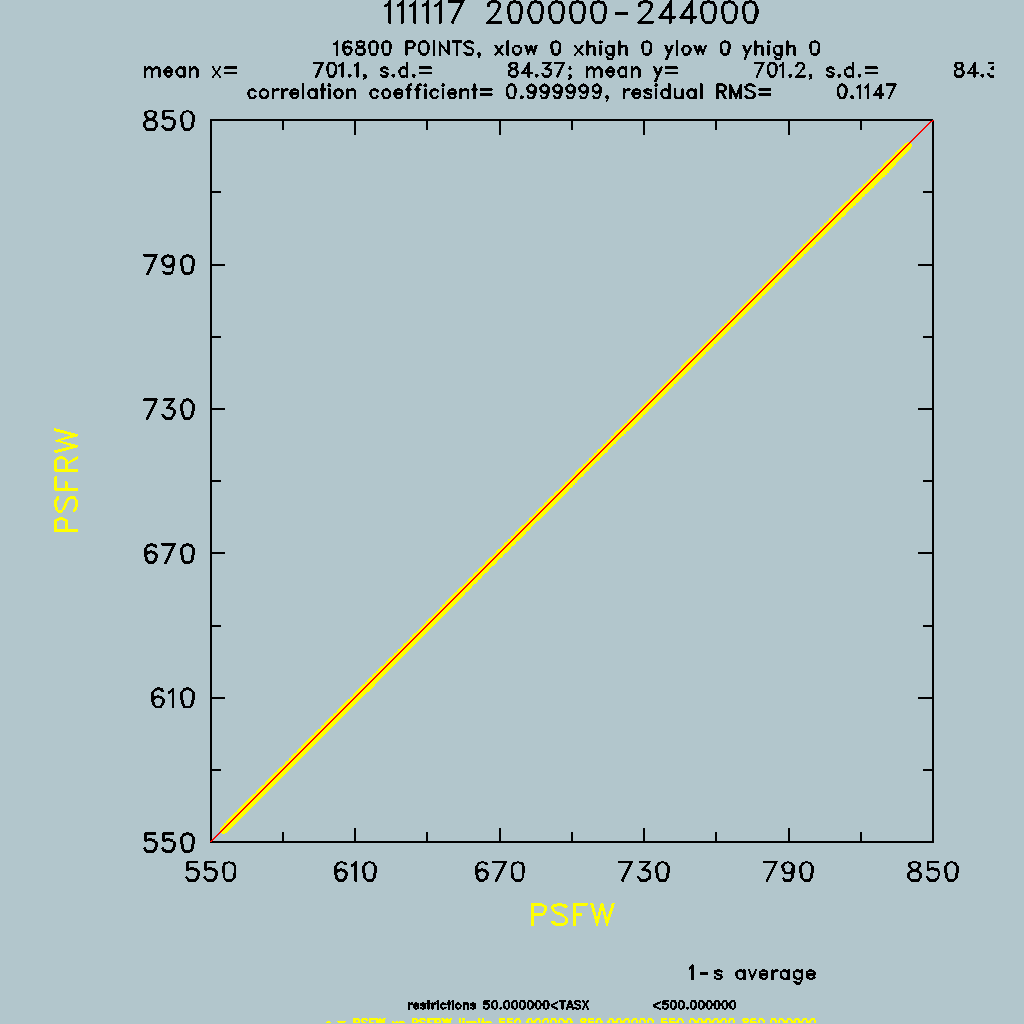
\includegraphics[width=6.5cm]{/home/cooperw/Xanadu/IDEAS/PcomparisonR8}
\par\end{center}


\lyxframeend{}\lyxframe{SOURCE OF NOISE?}
\begin{columns}%{}


\column{5 cm}
\begin{block}
{Coherence, 
TASF vs TAS\_LAMS}
\begin{itemize}
\item boundary layer flight segment
\item drops significantly by 5 Hz
\item only 0.9 at 0.2 Hz
\end{itemize}
\end{block}

\column{6.6 cm}
\begin{exampleblock}
{}

\begin{center}
\includegraphics[width=6.5cm]{/home/cooperw/Xanadu/IDEAS/COHERENCE}
\par\end{center}

\end{exampleblock}
\end{columns}%{}

\lyxframeend{}\lyxframe{VARIANCE SPECTRA}

\begin{center}
\includegraphics[width=6.5cm]{/home/cooperw/Xanadu/IDEAS/PSDmerged}
\par\end{center}


\lyxframeend{}\section{Flight Maneuvers}


\lyxframeend{}\subsection{Checking PCORs}


\lyxframeend{}\lyxframe{REVERSE-HEADING FLIGHT SEGMENTS}
\begin{summaryblock}
{Reverse-heading maneuvers flown on flight 5 of IDEAS-4:}

\noindent \begin{center}
{\footnotesize }%
\begin{tabular}{|c|c|c|c|c|c|c|}
\hline 
\textbf{\footnotesize Time Interval} & \textbf{\footnotesize UXW} & \textbf{\footnotesize GGTRK} & \textbf{\footnotesize THDG} & \textbf{\footnotesize WDC} & \textbf{\footnotesize WSC} & \textbf{\footnotesize UX}\tabularnewline
\hline 
\hline 
{\footnotesize 220000--230530} & {\footnotesize 1.56$\pm$0.91} & {\footnotesize 241} & {\footnotesize 242} & {\footnotesize 65 } & {\footnotesize 3.31 } & {\footnotesize 2.89}\tabularnewline
\hline 
{\footnotesize 230700--231200} & {\footnotesize -1.08$\pm$0.55} & {\footnotesize 59} & {\footnotesize 59} & {\footnotesize 224} & {\footnotesize 1.43} & {\footnotesize -1.47}\tabularnewline
\hline 
{\footnotesize 225100--225300} & {\footnotesize 1.975$\pm0.40$} & {\footnotesize 148} & {\footnotesize 149} & {\footnotesize 312} & {\footnotesize 2.58} & {\footnotesize 2.40 }\tabularnewline
\hline 
{\footnotesize 225500--225700} & {\footnotesize 0.99$\pm0.52$} & {\footnotesize 328} & {\footnotesize 329} & {\footnotesize 122} & {\footnotesize 1.09 } & {\footnotesize 1.21}\tabularnewline
\hline 
\end{tabular}
\par\end{center}{\footnotesize \par}

\end{summaryblock}
\begin{block}
{Test of Accuracy:\\
Longitudinal Wind Should Reverse}
\begin{itemize}
\item \textcolor{black}{Set \#1: $\Delta$UXW$\simeq$0.5 m/s (vs. 1.4 m/s,
std) }
\item \textcolor{red}{Set \#2: $\Delta\mathrm{UXW}\simeq3.0$ m/s (vs 3.6
m/s, std)}
\end{itemize}
\end{block}

\lyxframeend{}\subsection{Checking Layer Temperatures}


\lyxframeend{}\lyxframe{CALIBRATING TEMPERATURE USING LAMS}
\begin{block}
{Integrating the Hydrostatic Equation}
\begin{itemize}
\item Assumption: absolute pressure is accurate as calibrated, LAMS
\item GPS provides acurate measurement of geometric altitude
\item Integrate the hydrostatic equation between two pressure levels:

\begin{itemize}
\item Predicted altitude change depends on the ``mean'' temperature.
\item Comparison to a similar ``mean'' of the measurements checks the
accuracy of the temperature measurement.
\end{itemize}
\end{itemize}
\end{block}

\lyxframeend{}\lyxframe{EQUATIONS USED}
\begin{block}
{Three Sums Are Needed: $S_{1}$, $S_{2}$, $S_{3}$:}

\[
\delta p_{i}=-\frac{g\, p_{i}}{R_{a}T_{a,i}}\delta z_{i}\,\,\,\,\,\mathrm{(too\, noisy,\, second-by-second)}
\]



\[
S_{1}=\sum_{i}\frac{R_{a,i}}{g_{i}}\ln\left(\frac{p_{i}}{p_{i-1}}\right)
\]



\[
S_{2}=\sum_{i}(z_{i}-z_{i-1})
\]



\[
S_{3}=\sum_{i}\frac{z_{i}-z_{i-1}}{T_{m,i}}
\]


\end{block}
\begin{alertblock}
{Then compare prediction ($T_p$) to observed ($T_m$)}

\centerline{$T_{p}=-S_{1}/S_{2}$ and $\overline{T}_{m}=S_{2}/S_{3}$,
weighted appropriately}

\end{alertblock}

\lyxframeend{}\lyxframe{RESULTS FOR MEAN TEMPERATURES BETWEEN LAYERS}

\noindent \begin{center}
\vskip-1 cm%
\begin{minipage}[t]{1\columnwidth}%
\noindent \begin{center}
\begin{tabular}{|c|c|c|c|}
\hline 
Flight Segment & $T_{p}$ & $\overline{T}_{m}$ & $\Delta T$\tabularnewline
\hline 
\hline 
RF05, 205800--211100 & -10.98 & -10.37 & -0.5\tabularnewline
\hline 
RF07, 212510--213300 & -6.36 & -5.89 & -0.47\tabularnewline
\hline 
RF07, 212510--212900 & 2.27 & 2.42 & -0.15\tabularnewline
\hline 
RF07, 212900--213300 & -12.85 & -12.15 & -0.70\tabularnewline
\hline 
RF08, 214500--215300 & -0.9 & -0.5 & -0.4\tabularnewline
\hline 
RF08, 233700--234130 & -6.5 & -6.3 & -0.4\tabularnewline
\hline 
RF08, 234500--235000 & -9.4 & -8.8 & -0.6\tabularnewline
\hline 
RF08, 235600--240100 & -9.5 & -8.4 & -1.1\tabularnewline
\hline 
mean offset%
\footnote{excluding the first listed value for RF07 because the next two break
this climb segment into two segments%
}, $T_{p}-\overline{T}_{m}$ &  &  & \textcolor{red}{-0.55}\tabularnewline
\hline 
\end{tabular}
\par\end{center}%
\end{minipage}
\par\end{center}


\lyxframeend{}\section{LAMS-Based Temperature Measurement}


\lyxframeend{}\lyxframe{DETERMINING THE MACH NUMBER}
\begin{summaryblock}
{}

\textrm{\textcolor{none}{
\[
M^{2}=\left\{ \left(\frac{2c_{v}}{R_{a}}\right)\left[\left(\frac{p+q}{\mathrm{p}}\right)^{R_{a}/c_{p}}-1\right]\right\} 
\]
}}
\begin{itemize}
\item LAMS provides a correction $\Delta p$ to be added to $p$ and subtracted
from $q$ (affecting only the denominator). 
\item Measured temperature is not needed (except indirectly as it enters
fitting to find $\Delta p$).
\item Once calibrated, the above equation for $M^{2}$ can be used to find
the temperature, independent of a temperature probe, using only pressure
measurements and $v$ determined by LAMS::\\
\[
T_{LAMS}=v^{2}/(\gamma R_{a}M^{2})
\]

\end{itemize}
\end{summaryblock}

\lyxframeend{}\lyxframe{AN EXAMPLE OF T FROM LAMS}
\begin{exampleblock}
{}
\begin{overlayarea}
{11 cm}{6.0 cm}
\begin{onlyenv}%{}
<1->

\begin{center}
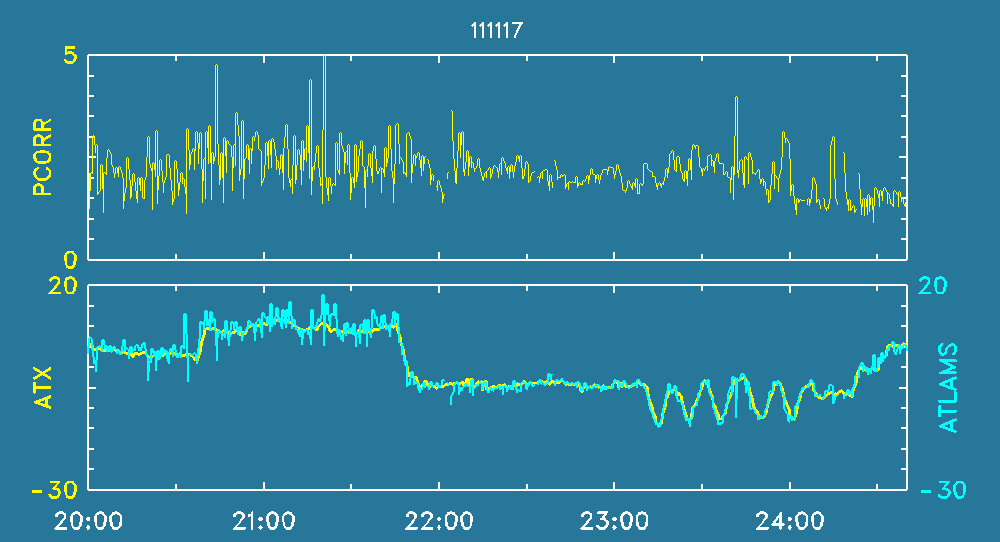
\includegraphics[width=11cm]{/home/cooperw/Xanadu/IDEAS/ATLAMS1}
\par\end{center}

\end{onlyenv}%{}


\begin{onlyenv}%{}
<2>
\begin{columns}%{}


\column{4 cm}


\column{5.5 cm}


\vskip-10cm
\begin{alertblock}
{Noise in the BL}
\begin{itemize}
\item $v$ from LAMS and $q$ from pitot tube measure different volumes
(cf.~coherence)
\item to use this, perhaps should filter $v$, $q$, or $T_{LAMS}$
\end{itemize}
\end{alertblock}
\end{columns}%{}
\end{onlyenv}%{}
\end{overlayarea}
\end{exampleblock}

\lyxframeend{}\section{Conclusions}
\begin{summaryblock}
{Key Results:}
\begin{enumerate}
\item LAMS provides a direct calibration of airspeed.

\begin{itemize}
\item TAS\_LAMS is slightly higher than TASX
\end{itemize}
\item This calibrates dynamic pressure:

\begin{itemize}
\item $q$ should be increased by about 0.5 mb on average.
\end{itemize}
\item If total pressure is accurately measured, this calibrates pressure:

\begin{itemize}
\item $p$ should be decreased by about 0.5 mb on average.
\end{itemize}
\item Accurate pressure supports integration of the hydrostatic equation
to calibrate temperature:

\begin{itemize}
\item Results indicate that temperature should be decreased by about 0.5$^{\circ}$C.
\end{itemize}
\item It is then possible to derive a new temperature measurement solely
from $p$, $q$, and $v_{LAMS}$. 
\end{enumerate}
\end{summaryblock}

\lyxframeend{}
\end{document}
